\loesung{

Recall that the formula for the coefficient of determination $R^2$ is:
\begin{align*}
	R^2 = 1-\frac{SSE_{LM}}{SSE_{c}} = 1 - \frac{\sum_{i=1}^n (y^{(i)} - \hat{f}_{LM}(x^{(i)}))^2}{\sum_{i=1}^n (y^{(i)} - \bar{y})^2}
	= 1 - \frac{\sum_{i=1}^n (y^{(i)} - \hat{y}^{(i)})^2}{\sum_{i=1}^n (y^{(i)} - \bar{y})^2}
\end{align*}
where $SSE_{LM} = \sum_{i=1}^n (y^{(i)} - \hat{f}_{LM}(x^{(i)}))^2$ is the sum of squares due to regression (error) and $SSE_{c} = \sum_{i=1}^n (y^{(i)} - \bar{y})^2$ is the total sum of squares. 

\begin{center}
	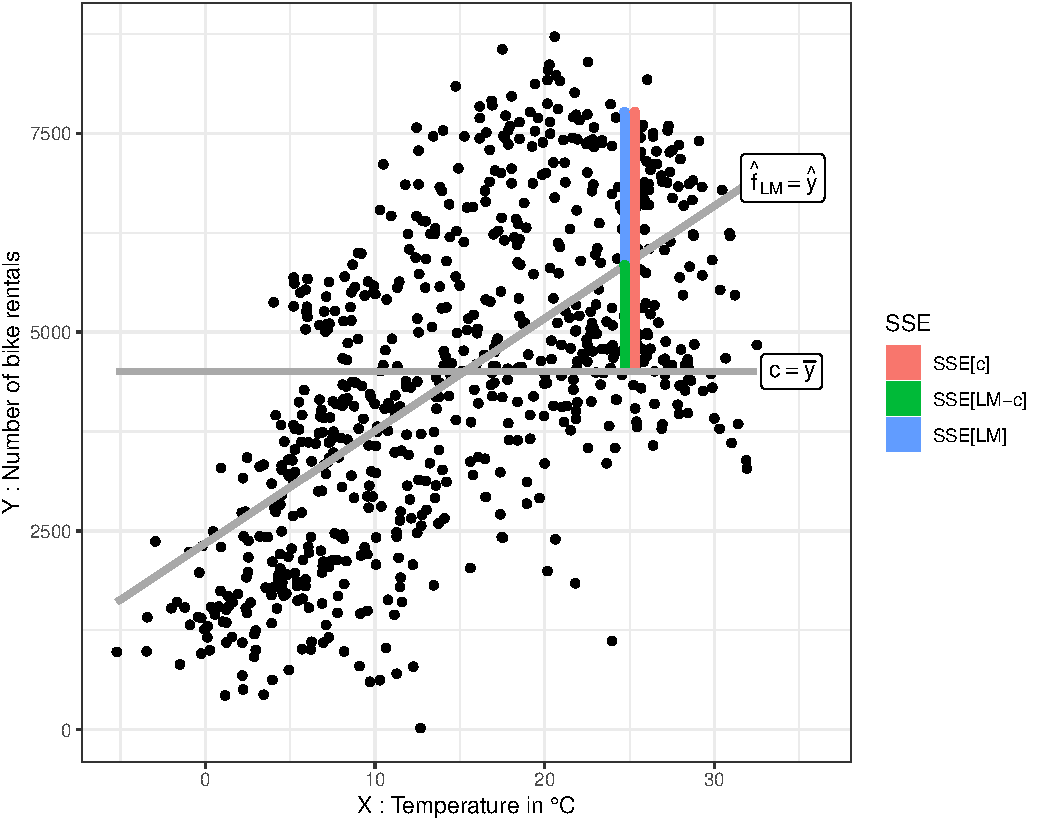
\includegraphics[width=0.75\maxwidth]{figure/r_squared.pdf}
\end{center}

First it is shown that 
\begin{align} \label{P2}
	R^2 = 1-\frac{SSE_{LM}}{SSE_{c}} = 1 - \frac{\sum_{i=1}^n (y^{(i)} - \hat{y}^{(i)})^2}{\sum_{i=1}^n (y^{(i)} - \bar{y})^2}
	= \frac{\sum_{i=1}^n (\hat{y}^{(i)} - \bar{y})^2}{\sum_{i=1}^n (y^{(i)} - \bar{y})^2} = \frac{SSE_{LM-c}}{SSE_{c}}
\end{align}

\fbox{\parbox{\linewidth}{
		
Note that

\begin{align} \label{P1}
	\sum_{i=1}^n (y^{(i)}-\bar{y})^2 &= \sum_{i=1}^n (y^{(i)}-\hat{y}^{(i)})^2 + \sum_{i=1}^n (\hat{y}^{(i)} - \bar{y})^2.
\end{align}
Proof: 
\begin{align*}
	\sum_{i=1}^n (y^{(i)}-\bar{y})^2 
	&= \sum_{i=1}^n (y^{(i)} - \hat{y}^{(i)} + \hat{y}^{(i)} - \bar{y})^2 \\
	&= \sum_{i=1}^n (y^{(i)} - \hat{y}^{(i)})^2 + (\hat{y}^{(i)} - \bar{y})^2 + 2(y^{(i)}-\hat{y}^{(i)})(\hat{y}^{(i)} - \bar{y}) \\
	&= \sum_{i=1}^n (y^{(i)} - \hat{y}^{(i)})^2 + \sum_{i=1}^n(\hat{y}^{(i)} - \bar{y})^2 + 2\sum_{i=1}^n(y^{(i)}-\hat{y}^{(i)})(\hat{y}^{(i)} - \bar{y})
\end{align*}}}
\fbox{\parbox{\linewidth}{
		
It remains to show that 
\begin{align*}
	2\sum_{i=1}^n(y^{(i)}-\hat{y}^{(i)})(\hat{y}^{(i)} - \bar{y}) &= 0 \\
	\sum_{i=1}^n (y^{(i)}-\hat{y}^{(i)})\hat{y}^{(i)} - \sum_{i=1}^n (y^{(i)}-\hat{y}^{(i)})\bar{y}&= 0 \\
	\bar{y}\, \sum_{i=1}^n y^{(i)}-\hat{y}^{(i)} &= 0 \\
	\sum_{i=1}^n y^{(i)}-\hat{y}^{(i)} &= 0
\end{align*}

where we have used the fact that $\sum_{i=1}^n (y^{(i)}-\hat{y}^{(i)})\hat{y}^{(i)} = 0$ as the residuals $(y^{(i)}-\hat{y}^{(i)})$ and $\hat{y}^{(i)}$ are not correlated. 

\hfill (proof of (\ref{P1})) $\Box$ \\
}}

\bigskip

It follows: 
\begin{align*}
	R^2 &=  1 - \frac{\sum_{i=1}^n (y^{(i)} - \hat{y}^{(i)})^2}{\sum_{i=1}^n (y^{(i)} - \bar{y})^2} 
	= \frac{\sum_{i=1}^n (y^{(i)} - \bar{y})^2 - \sum_{i=1}^n (y^{(i)} - \hat{y}^{(i)})^2}{\sum_{i=1}^n (y^{(i)} - \bar{y})^2}\\
	&= \frac{\sum_{i=1}^n (y^{(i)}-\hat{y}^{(i)})^2 + \sum_{i=1}^n (\hat{y}^{(i)} - \bar{y})^2 - \sum_{i=1}^n (y^{(i)} - \hat{y}^{(i)})^2}{\sum_{i=1}^n (y^{(i)} - \bar{y})^2}
	= \frac{\sum_{i=1}^n (\hat{y}^{(i)} - \bar{y})^2}{\sum_{i=1}^n (y^{(i)} - \bar{y})^2}
\end{align*}
\hfill (proof of (\ref{P2})) $\Box$ \\ 

And further: 
\begin{align*}
	R^2 &= \frac{\sum_{i=1}^n (\hat{y}^{(i)} - \bar{y})^2}{\sum_{i=1}^n (y^{(i)} - \bar{y})^2}
	= \frac{\sum_{i=1}^n(\hat{\beta}_0 + \hat{\beta}_1 x^{(i)}- (\hat{\beta}_0 + \hat{\beta}_1 \bar{x}))^2}{\sum_{i=1}^n (y^{(i)} - \bar{y})^2}
	= \frac{\hat{\beta}_1^2 \sum_{i=1}^n (x^{(i)} - \bar{x})^2}{\sum_{i=1}^n (y^{(i)} - \bar{y})^2} 
\end{align*}

Now, starting with $\rho^2$, we can write:
\begin{align*}
	\rho^2 &= \left(\frac{\sum_{i=1}^n (x^{(i)} - \bar{x})(y^{(i)} - \bar{y})}{\sqrt{\sum_{i=1}^n (x^{(i)} - \bar{x})^2}\sqrt{\sum_{i=1}^n (y^{(i)} - \bar{y})^2}}\right)^2 \\
	&= \frac{\left(\sum_{i=1}^n (x^{(i)} - \bar{x})(y^{(i)} - \bar{y})\right)^2}{\sum_{i=1}^n (x^{(i)} - \bar{x})^2\sum_{i=1}^n (y^{(i)} - \bar{y})^2}\\
	&= \frac{\left(\sum_{i=1}^n (x^{(i)} - \bar{x})(y^{(i)} - \bar{y})\right)^2}{\sum_{i=1}^n (x^{(i)} - \bar{x})^2\sum_{i=1}^n (y^{(i)} - \bar{y})^2} \frac{\sum_{i=1}^n (x^{(i)} - \bar{x})^2}{\sum_{i=1}^n (x^{(i)} - \bar{x})^2}\\
	&= \left(\frac{\sum_{i=1}^n (x^{(i)} - \bar{x})(y^{(i)} - \bar{y})}{\sum_{i=1}^n (x^{(i)} - \bar{x})^2}\right)^2 \frac{\sum_{i=1}^n (x^{(i)} - \bar{x})^2}{\sum_{i=1}^n (y^{(i)} - \bar{y})^2} \\
	&= \hat{\beta}_1^2 \, \frac{\sum_{i=1}^n (x^{(i)} - \bar{x})^2}{\sum_{i=1}^n (y^{(i)} - \bar{y})^2}
	= R^2
\end{align*}

%$\Rightarrow R^2 = \rho^2$.
%
%\bigskip
%
%\textbf{Option 2:}
%\begin{align*}
%	R^2 &= 1 - \frac{SSE_{LM}}{SSE_{c}} = 1 - \frac{\sum_{i=1}^n (y^{(i)} - \hat{y}^{(i)})^2}{\sum_{i=1}^n (y^{(i)} - \bar{y})^2} \\
%	&= \frac{\sum_{i=1}^n (\hat{y}^{(i)} - \bar{y})^2}{\sum_{i=1}^n (y^{(i)} - \bar{y})^2} 
%\end{align*}

Hence, we have shown that $R^2 = \rho^2$, which completes the proof. Note that this result is valid only for simple linear regression, where there is only one independent variable. For multiple regression, the coefficient of determination is defined differently and does not necessarily equal the square of the Pearson correlation coefficient.

\hfill $\Box$ \\
\vspace*{-0.3cm}
}
